\documentclass[12pt,letterpaper]{article}
\usepackage[left=1in,top=1in,right=1in,bottom=1in,nohead]{geometry}
\pagestyle{empty}
\linespread{1.5}
\usepackage[T1]{fontenc}
\usepackage{ragged2e}
\usepackage{setspace}
\usepackage{mdwlist}
% \usepackage{array}
% \usepackage{multirow}
\usepackage{graphicx}
% \usepackage{wrapfig}
% \usepackage{longtable}
% \usepackage{subfig}
\usepackage{amsmath}
\usepackage{amssymb}
\usepackage{bbm}
\usepackage{dsfont}
\usepackage{mathptmx}
\usepackage[hang]{caption}
\DeclareMathAlphabet{\mathcal}{OMS}{cmsy}{m}{n}
\usepackage{relsize}
\usepackage{fancyvrb}
\def \fullline {\vspace{.2em}\hrule\vspace{3px}}

\begin{document}
\tableofcontents
\setlength{\parindent}{0.25in}
\setlength{\floatsep}{0in}
\section{Radial Density Function}
\subsection{Calculation of Distances with Periodicity}
Suppose a large chemical structure has uncountably many atoms but the follow a
periodic pattern of $n$ atoms every $p$ Angstroms. The atom locations within a
period are given by $a_1, a_2, \ldots, a_n$ where $a_i \in \mathbb{R}^3$. The
radial density function is the distribution of pairwise distances between these
atoms.

The distances $d$ between atoms $a_i$ and $a_j$ where $i \neq j$, atom $a_i$
has been displaced by $x$, and atom $a_j$ has been displaced by $y$ per the
periodicity is 
\begin{align*}
  d^2 &= \langle a_i + x - (a_j + y), a_i + x - (a_j + y) \rangle \\
      &= \langle a_i-a_j, a_i-a_j \rangle  + \langle x-y, x-y \rangle  
      + 2 \langle a_i-a_j,x-y \rangle 
\end{align*}
where $x =(k_1 p, k_2 p, k_3 p)$ for $k_i \in \mathbb{Z}$ 
and $y = (l_1 p, l_2 p, l_3 p)$ for $l_i \in \mathbb{Z}$.
Here $\langle x,y \rangle $ denotes the inner product between $x$ and $y$. 

Suppose $D$ is a random variable that samples at random the distances, $d$, in
the chemical structure. The radial density function is the probability density
function of this random variable. This function can be estimated empirically via
a histogram.

The histogram is then normalized by the volume a spherical shell.
\begin{align*}
  \frac{4}{3} &\pi (r + \Delta r)^3 - \frac{4}{3} \pi r^3\\
     &=\frac{4}{3} (3 r^2 \Delta r + 3 r (\Delta r)^2 + (\Delta r)^3) \\
              &\approx 4 \pi r^2 \Delta r
\end{align*}
where $\Delta r$ tends to zero.

For a histogram with frequency, $f$, for bin $[d_i, d_{i+1}]$, we replace $f$
with $f / d_i^2$. And then normalize the histogram so that the sum over all bins
is one.

\subsection{Adding Noise For Atom Vibration}
Due to the vibrations of the molecules, the radial density function will not be
just the equilibrium positions. We can approximate this fluctuation in distances
via a Gaussian filter or Weierstrass transform.

\begin{align*}
F(x)=\frac{1}{\sqrt{4\pi t}} 
  \int_{-\infty}^\infty f(y) e^{-\frac{(x-y)^2}{4t}} dy
\end{align*}

Given that the density function is only defined for a finite number of
distances, we use a discrete version of the transform making sure to keep the
sum of the weights equal to one.

\begin{align*}
  F(d_k) = \frac{\sum_{d_i = d_0}^{d_n} f(d_i) \exp\left(-\frac{(d_k -
                  d_i)^2}{4t}\right)}
            {\sum_{d_i = d_0}^{d_n} \exp\left(-\frac{(d_k - d_i)^2}{4t}\right)}
\end{align*}
where $d_0$ is the minimum distance and $d_n$ is the maximum distance.

\subsection{Cubane Example}
As an example of the above, below are the calculations for cubane ($C_8 H_8$).\\

\noindent Here are the coordinates of the elements in cubane in Angstroms.

\begin{verbatim}
Element, x, y, z
C, 1.2455, 0.5367,-0.0729
C, 0.9239,-0.9952, 0.0237
C,-0.1226,-0.7041, 1.1548
C, 0.1989, 0.8277, 1.0582
C, 0.1226, 0.7042,-1.1548
C,-0.9239, 0.9952,-0.0237
C,-1.2454,-0.5367, 0.0729
C,-0.1989,-0.8277,-1.0582
H, 2.2431, 0.9666,-0.1313
H, 1.6638,-1.7924, 0.0426
H,-0.2209,-1.2683, 2.0797
H, 0.3583, 1.4907, 1.9059
H, 0.2208, 1.2681,-2.0799
H,-1.6640, 1.7922,-0.0427
H,-2.2430,-0.9665, 0.1313
H,-0.3583,-1.4906,-1.9058
\end{verbatim}

\subsubsection{Cubane Radial Density Functions}
\begin{figure}[ht!]
  \begin{center}
    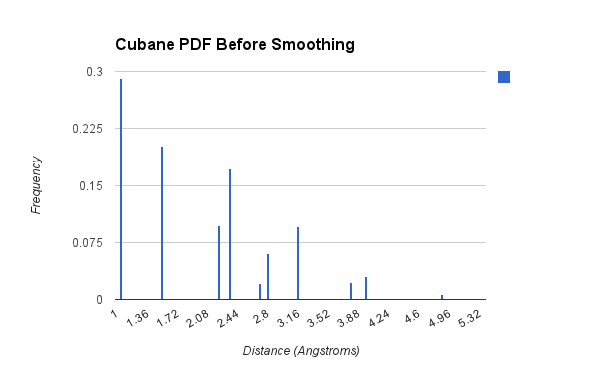
\includegraphics[scale=0.7]{figs/cubane_rdf_before_smoothing.png}
    \caption{Before Smoothing}
  \end{center}
\end{figure}

\begin{figure}[ht!]
  \begin{center}
    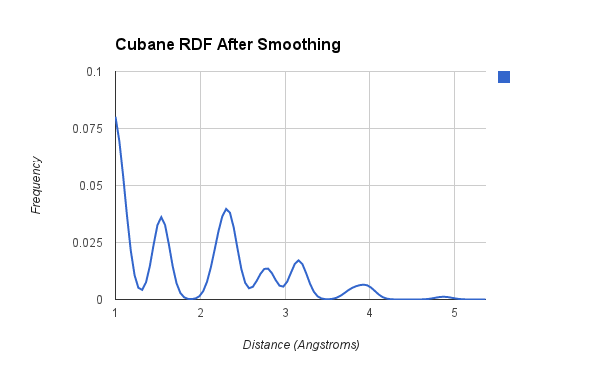
\includegraphics[scale=0.7]{figs/cubane_rdf_after_smoothing.png}
    \caption{After Smoothing}
  \end{center}
\end{figure}
\clearpage

\subsection{Experimental and Theoretical RDFs for Known Structures}
For some structures, we are able to theoretically calculate the RDF from atom
locations and also have the experimental RDF from Xray scattering. These known
matches provide some insight into understanding how the experiments and theory
align. The RDF comparison are shown below.

Outside of these structures, there are not many other known matches. There are a
few reasons for this. First, if a structures is already known at the atomic
level then there is no need to run an xray diffraction experiment. Second, if a
structure is periodic as in a lattice, the atomic structure can be determined by
xray diffraction which is easier and cheaper than xray scattering.

\subsubsection{Ga As}
\noindent Experimental Data: Pair Distribution Functions Analysis, Valeri
Petkov\\
\noindent Calculated Data: Maria Chan\\
\begin{figure}[ht]
  \begin{center}
    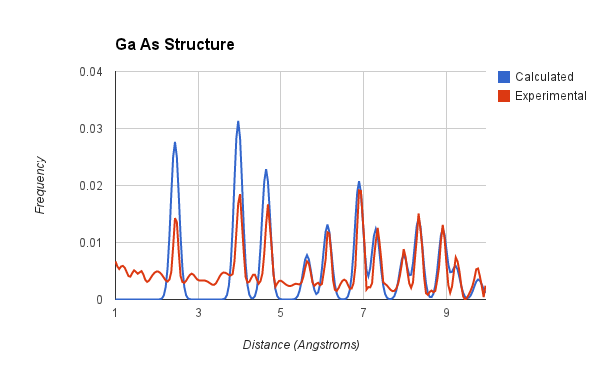
\includegraphics[scale=0.7]{figs/gaas_rdf_comparison.png}
    \caption{Ga As}
  \end{center}
\end{figure}

\subsubsection{In As}
\noindent Experimental Data: Pair Distribution Functions Analysis, Valeri
Petkov\\
\noindent Calculated Data: Maria Chan\\
\begin{figure}[ht]
  \begin{center}
    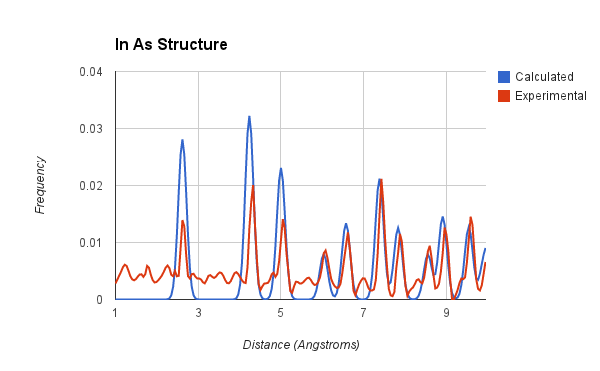
\includegraphics[scale=0.7]{figs/inas_rdf_comparison.png}
    \caption{In As}
  \end{center}
\end{figure}

\subsubsection{Si Lattice}
\noindent Experimental Data: J. AM. CHEM. SOC. VOL. 133, NO. 3, 2011, P:
503-512\\
\noindent Calculated Data: http://materialsproject.org/materials/mp-149/ \\
\begin{figure}[ht]
  \begin{center}
    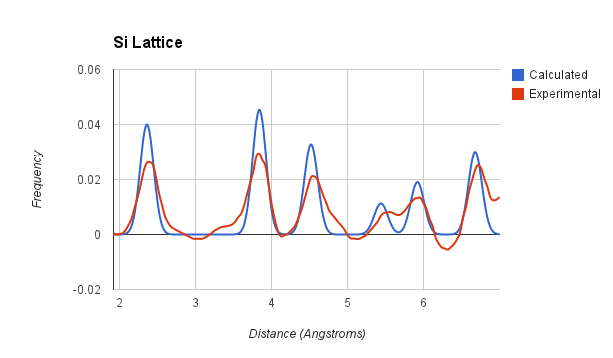
\includegraphics[scale=0.7]{figs/si_lattice_comparison.png}
    \caption{Si Lattice}
  \end{center}
\end{figure}

\pagebreak

\section{Principal Component Analysis}
\subsection{Data Set}
For the analysis following, a data set of radial density functions was used that
contained 3,491 theoretical SiLi structures, 8 experimental SiLi structures, a
pair of theoretical and calculated GaAs structures, and a pair of theoretical and
calculated InAs structures. Each image had 128 evenly distances from 1.92 to
7 angstroms.

\subsection{Dimensionality}
To discover the minimal dimensionality of the RDF data, I charted the cumulative
proportion of variance explained by adding successive principal components. We
can see from Figure $\ref{f:pca_dim}$ that around 30 principal components explain
99\% of the variance. 

\begin{figure}[ht]
  \begin{center}
    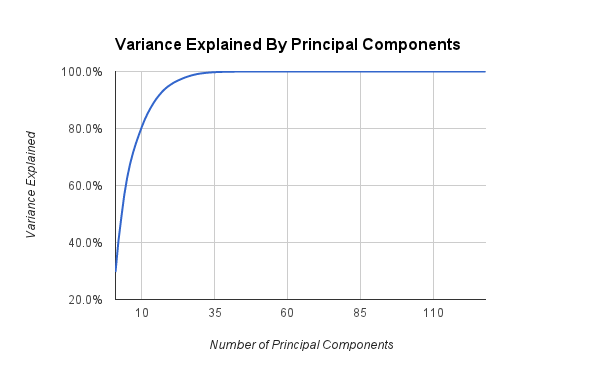
\includegraphics[scale=0.7]{figs/pca_proportion_variance.png}
    \caption{Proportion of Variance Explained\label{f:pca_dim}}
  \end{center}
\end{figure}

\subsection{Basis Vectors}
Sometimes PCA analysis gives intelligible basis vectors that identify a key
characteristic in the data set. In the case of the RDF images, the basis vectors
appear to be nonsensical. The first four principal component basis vectors are
show in Figure $\ref{f:pca_basis}$.

\begin{figure}[ht]
  \begin{center}
    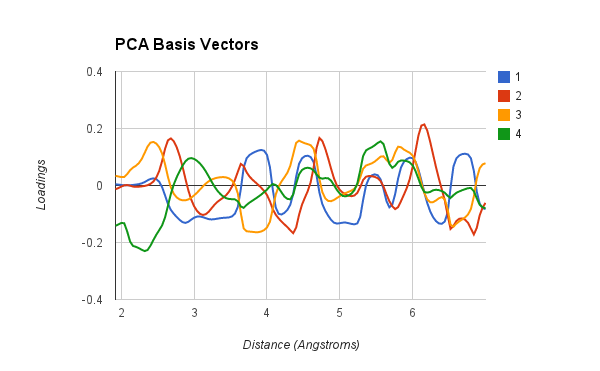
\includegraphics[scale=0.7]{figs/pca_basis_vectors.png}
    \caption{PCA Basis Vectors\label{f:pca_basis}}
  \end{center}
\end{figure}
\clearpage

\subsection{Projected RDFs}
To further assess the capacity of PCA to reduce the dimensionality of the data,
I sampled a few images and projected them onto PCA space with decreasing
dimensions.

\subsubsection{SiLi Calc10136}
\begin{figure}[ht]
  \begin{center}
    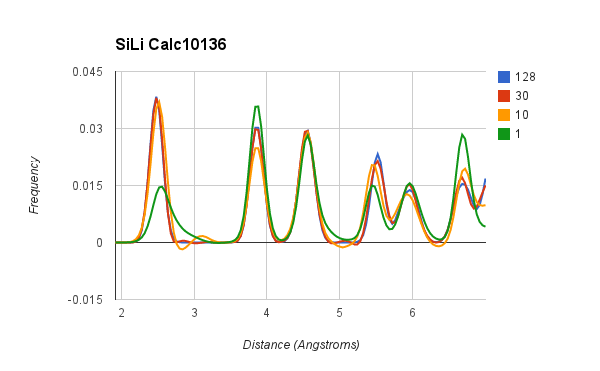
\includegraphics[scale=0.7]{figs/pca_proj_sili_calc10136.png}
    \caption{SiLi Calc10136 Projections}
  \end{center}
\end{figure}
\clearpage

\subsubsection{SiLi Expt1}
\begin{figure}[ht]
  \begin{center}
    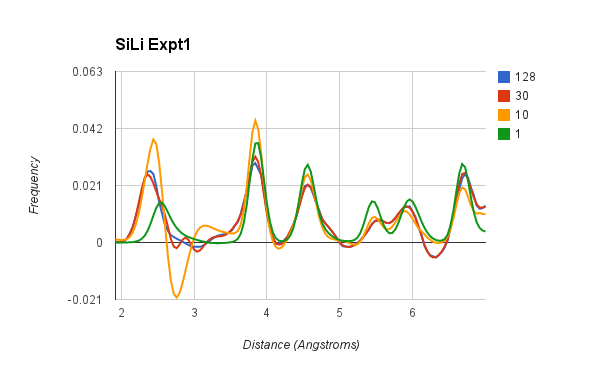
\includegraphics[scale=0.7]{figs/pca_proj_sili_expt1.png}
    \caption{SiLi Expt1 Projections}
  \end{center}
\end{figure}
\clearpage

\subsubsection{SiLi Expt8}
\begin{figure}[ht]
  \begin{center}
    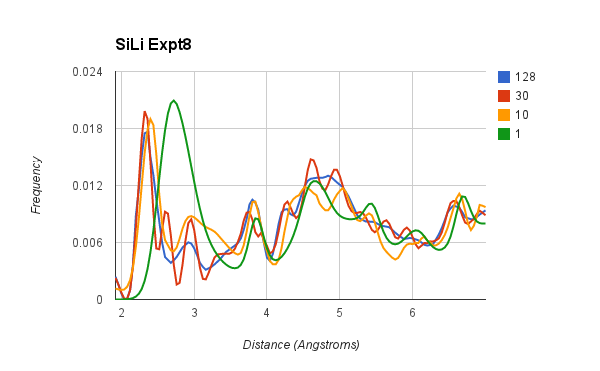
\includegraphics[scale=0.7]{figs/pca_proj_sili_expt8.png}
    \caption{SiLi Expt8 Projections}
  \end{center}
\end{figure}
\clearpage

\subsubsection{GaAs Expt}
\begin{figure}[ht]
  \begin{center}
    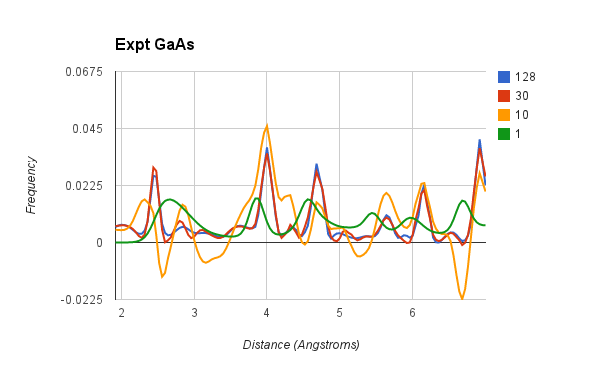
\includegraphics[scale=0.7]{figs/pca_proj_gaas_expt.png}
    \caption{GaAs Expt Projections}
  \end{center}
\end{figure}
\clearpage

\subsection{Observations}
From the proportion of variance explained and the selected projections, clearly
thirty principal components are sufficient to capture the essence of the image.
Also, it shows that one principal component is not sufficient in most cases. It
is strange however that the first principal component captures so clearly
SiLi Calc10136. Further investigation is needed to determine whether this is due
the large number of images similar to Calc10136 in the data set.

\section{Noise Analysis}
% exp noise example
% peak counts: estimation method, histogram, dist
% peak location: estimation method, histogram, dist
% noise peak heights: estimation method, histogram, dist
% example noisy images
% peak counts for max lengths
\subsection{Peak Counts}
\begin{figure}[ht]
  \begin{center}
    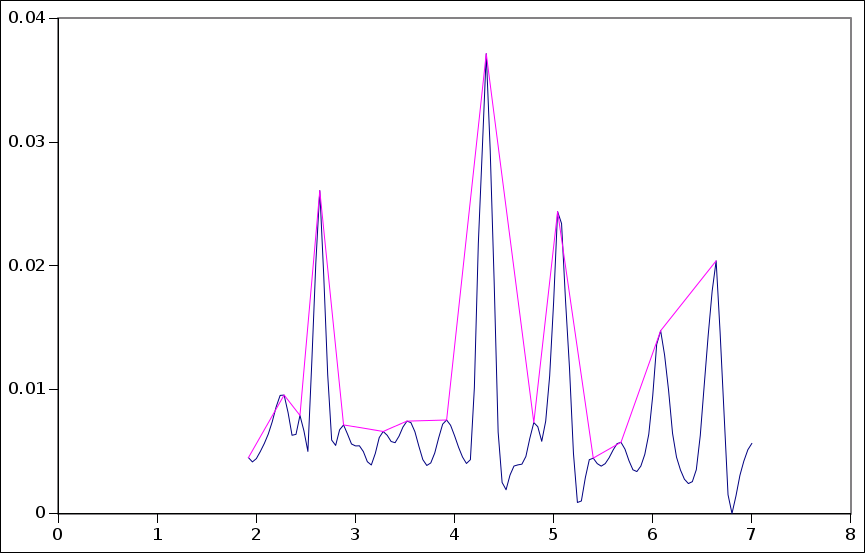
\includegraphics[scale=0.5]{figs/inas_peaks_7ang.png}
    \caption{InAs Expt, Max 7 Angstroms}
  \end{center}
\end{figure}

\begin{figure}[ht]
  \begin{center}
    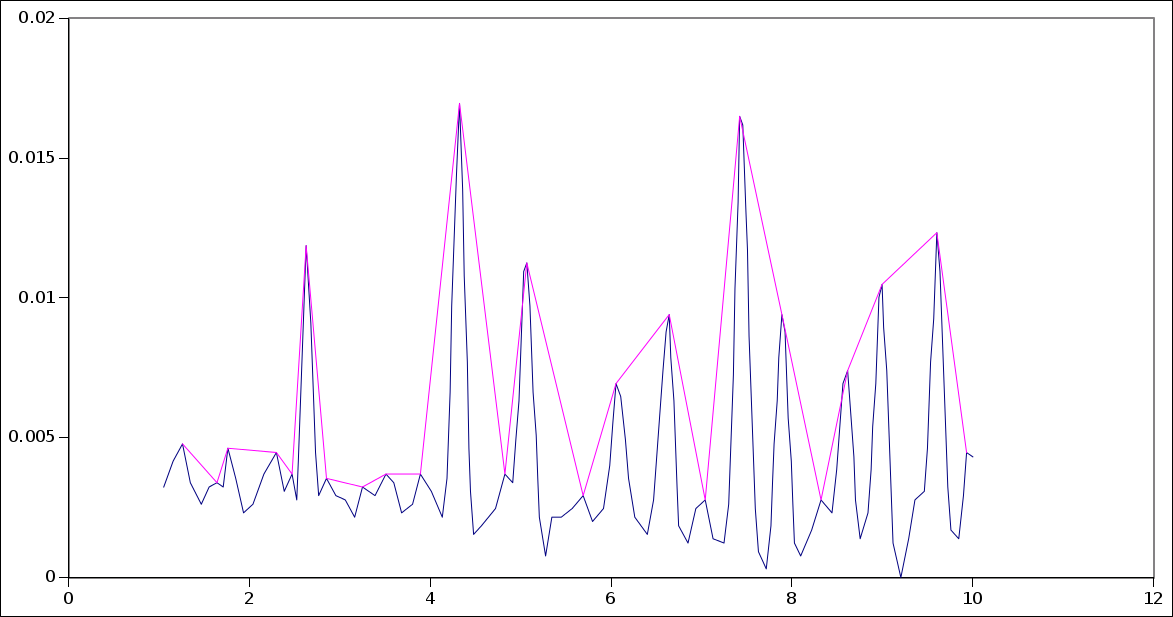
\includegraphics[scale=0.4]{figs/inas_peaks_10ang.png}
    \caption{InAs Expt, Max 10 Angstroms}
  \end{center}
\end{figure}
\clearpage

\section{Sources}
\begin{verbatim}
http://en.wikipedia.org/wiki/Atom_vibrations
http://en.wikipedia.org/wiki/Radial_distribution_function
http://en.wikipedia.org/wiki/Weierstrass_transform
http://matplotlib.org/api/mlab_api.html
\end{verbatim}

%\pagebreak
%\noindent \textbf{Appendix}\\
%\emph{Convolution Commutativity}\\
%\begin{align*}
%&\int_{- \infty}^\infty f(\tau) g(t - \tau) d\tau\\
%&u = t - \tau\\
%&\tau = -\infty \rightarrow u = \infty\\
%&\tau = \infty \rightarrow u = -\infty\\
%&du = -d\tau\\
%&- \int_\infty^{-\infty} f(t - u) g(u) du = \int_{-\infty}^\infty g(u) f(t-u)du\\
%\end{align*}

\end{document}
